\section{Birthsigns}
The people of Tamriel mark their calendars by the passage of constellations overhead. When the sun passes near one, it is that constellation's season. There are thirteen in total: one for each month of the year and then one which seems to wander intermittently, giving it no predictable season. This collection of constellations is known as the Firmament, and many attribute personality traits to the sign under which one was born. The signs of the Firmament are listed here in chronological order; each one grants a certain bonus which may include attribute increases and powers.

\begin{longtable}{lm{0.6\textwidth}}
	\raisebox{-0.5\height}{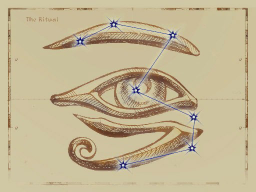
\includegraphics[width=0.3\textwidth]{Ritual.png}} & \textbf{The Ritual}: The month of Morning Star is marked by the Ritual, a sign denoting a deep connection with the moons and the Divines. Those born under the ritual gain two powers: Mara's Gift (allows them to heal themselves for 200 their health once a day) and Blessed Word (causes undead to flee for 3 rounds for 40 magicka).\\
	
	\raisebox{-0.5\height}{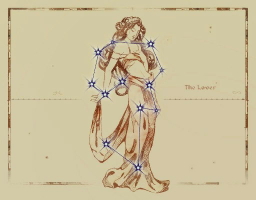
\includegraphics[width=0.3\textwidth]{Lover.png}} & \textbf{The Lover}: Those born in the month of Sun's Dawn under the Lover are said to be passionate and graceful. The Lover bestows the Lover's Kiss power, which allows the user to paralyze a target on touch for one round at the cost of 120 stamina damage.\\

	\raisebox{-0.5\height}{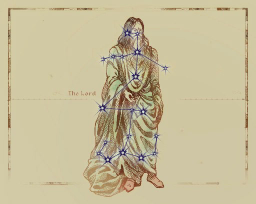
\includegraphics[width=0.3\textwidth]{Lord.png}} & \textbf{The Lord}: The Lord marks the month of First Seed, where he oversees all the planting in Tamriel. Those born under the Lord are said to be healthier than usual and are granted the Blood of the North power, allowing them to heal 45 health per round for 2 rounds at the cost of 50 magicka. However, they are also cursed with Troll's Blood, giving them a 25\% weakness to fire.\\

	\raisebox{-0.5\height}{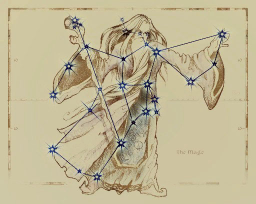
\includegraphics[width=0.3\textwidth]{Mage.png}} & \textbf{The Mage}: One of the three guardian signs, the Mage marks the month of Rain's Hand, when magicka was first used by humans. Those born under the Mage are particularly gifted in the arcane arts and gain a permanent +50 bonus to maximum magicka.\\

	\raisebox{-0.5\height}{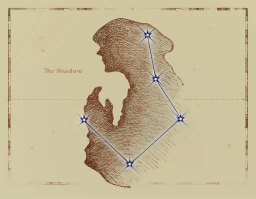
\includegraphics[width=0.3\textwidth]{Shadow.png}} & \textbf{The Shadow}: The Shadow's season is the month of Second Seed. This sign grants those born under it the power of Moonshadow, which lets them turn invisible for one minute, once a day.\\

	\raisebox{-0.5\height}{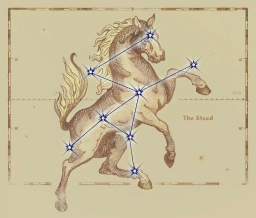
\includegraphics[width=0.3\textwidth]{Steed.png}} &
\textbf{The Steed}: Those born in the month of Mid Year under the sign of the Steed are impatient, always hurrying from place to place and restless whenever they have to wait. They gain a permanent +20 bonus to their Speed attribute.\\

\raisebox{-0.5\height}{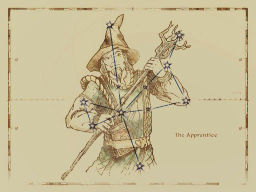
\includegraphics[width=0.3\textwidth]{Apprentice.png}} & \textbf{The Apprentice}: The month of Sun's Height is the season of the Apprentice. Those born under this sign are especially gifted with magic and gain a permanent +100 to max magicka; however, they also gain a permanent 100\% vulnerability to magic.\\

\raisebox{-0.5\height}{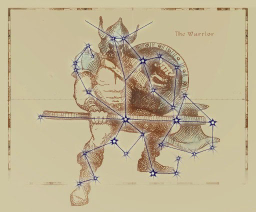
\includegraphics[width=0.3\textwidth]{Warrior.png}} & \textbf{The Warrior}: The Warrior is another of the guardian signs. It marks the month of Last Seed and is said to grant those born in this month skill with weapons of all kinds as well as a short temper. This sign grants a permanent +10 bonus to both Endurance and Strength.\\

\raisebox{-0.5\height}{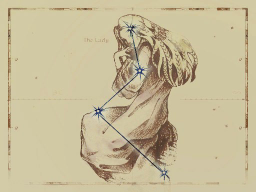
\includegraphics[width=0.3\textwidth]{Lady.png}} & \textbf{The Lady}: The Lady presides graciously over the month of Heartfire. Those born under this sign are said to be kind and tolerant, and they gain a permanent +10 bonus to both Willpower and Endurance.\\

\raisebox{-0.5\height}{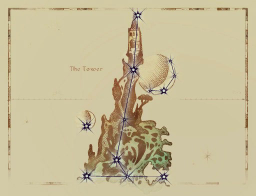
\includegraphics[width=0.3\textwidth]{Tower.png}} & \textbf{The Tower}: The Tower is a birthsign of great fortune, and those born under it are said to find treasure in one way or another. The Tower grants two powers: Tower Key (open a lock of average level or lower for free once a day) and Tower Warden (5\% chance to reflect incoming damage back to the target for 1 minute).\\

\raisebox{-0.5\height}{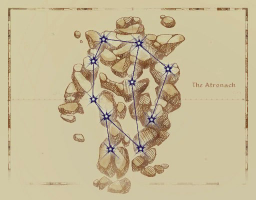
\includegraphics[width=0.3\textwidth]{Atronach.png}} & \textbf{The Atronach}: A sign representing elemental beings from Oblivion, the Atronach is both a blessing and a curse to aspiring mages. Those born under the Atronach gain a permanent +150 bonus to maximum magicka and have a 50\% chance to absorb spells targeting them (meaning they have no effect and you gain the magicka used to cast the spell). However, they cannot regenerate magicka on their own.\\

\raisebox{-0.5\height}{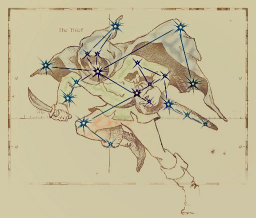
\includegraphics[width=0.3\textwidth]{Thief.png}} & \textbf{The Thief}: The final month of the year is Evening Star, and it is marked by the guardian sign of the Thief. Those born under the Thief are not necessarily thieves; instead, they are prone to risky lifestyles and rarely come to harm due to their natural luck. They receive a permanent +10 bonus to both Speed and Agility.\\

\raisebox{-0.5\height}{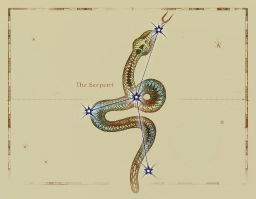
\includegraphics[width=0.3\textwidth]{Serpent.png}} & \textbf{The Serpent}: There are no common characteristics amongst those born under the Serpent, but they are said to be the most blessed and the most cursed. The Serpent grants the power of Serpent Spell, which has the following effects: the user may touch a target and damage them for 30 health per round for 2 rounds; whether or not a target is touched, the user is cured of poison, all magical effects of Expert level or lower are dispelled, and 100 stamina points are lost. This power may be used once per day.\\
\end{longtable}